\documentclass[final]{fhnwreport}       %[mode] = draft or final
                                        %{class} = fhnwreport, article, 
                                        %          report, book, beamer, standalone
%%---Main Packages-----------------------------------------------------------------------
\usepackage[english, ngerman]{babel}	%Mul­tilin­gual sup­port for LaTeX
\usepackage[T1]{fontenc}				%Stan­dard pack­age for se­lect­ing font en­cod­ings
\usepackage[utf8]{inputenc}				%Ac­cept dif­fer­ent in­put en­cod­ings
\usepackage{lmodern}                    %The newer Font-Set
\usepackage{textcomp}					%LaTeX sup­port for the Text Com­pan­ion fonts
\usepackage{caption}					%Customising captions in floating environments
\usepackage{graphicx} 					%En­hanced sup­port for graph­ics
\usepackage{float}						%Im­proved in­ter­face for float­ing ob­jects
\usepackage{ifdraft}                    %Let you check if the doc is in draft mode

%%---Useful Packages---------------------------------------------------------------------
\usepackage{color}						%Colour control for LaTeX documents
\usepackage[pdftex,dvipsnames]{xcolor}  %Driver-in­de­pen­dent color ex­ten­sions for LaTeX
\usepackage{csquotes}                   %Simpler quoting with \enquote{}
\usepackage{siunitx} 					%A com­pre­hen­sive (SI) units pack­age
\usepackage{listings}					%Type­set source code list­ings us­ing LaTeX
\usepackage[bottom]{footmisc}			%A range of foot­note op­tions
\usepackage{footnote}					%Im­prove on LaTeX's foot­note han­dling
\usepackage{verbatim}					%Reim­ple­men­ta­tion of and ex­ten­sions to LaTeX ver­ba­tim
\usepackage[textsize=footnotesize]{todonotes} %Mark­ing things to do in a LaTeX doc­u­ment
\usepackage{titling}					%Control over the typesetting of the \maketitle command

%%---Tikz Packages-----------------------------------------------------------------------
\usepackage{standalone}
\usepackage{tikz}
\usepackage{circuitikz}
\usetikzlibrary{arrows}
\usetikzlibrary{calc}
\usetikzlibrary{intersections}

%%---Math Packages-----------------------------------------------------------------------
\usepackage{amsmath}					%AMS math­e­mat­i­cal fa­cil­i­ties for LaTeX
\usepackage{amssymb}					%Type­set­ting symbols (AMS style)
%\usepackage{amstext}
%\usepackage{amsfonts}
%\usepackage{breqn}
\usepackage{array}						%Ex­tend­ing the ar­ray and tab­u­lar en­vi­ron­ments
\usepackage{amsthm}					%Type­set­ting the­o­rems (AMS style)

%%---Table Packages----------------------------------------------------------------------
\usepackage{tabularx}					%Tab­u­lars with ad­justable-width columns
%\usepackage{longtable}
\usepackage{multirow}					%Create tab­u­lar cells span­ning mul­ti­ple rows
\usepackage{multicol}					%In­ter­mix sin­gle and mul­ti­ple columns

%%---PDF / Figure Packages---------------------------------------------------------------
\usepackage{pdfpages}					%In­clude PDF doc­u­ments in LaTeX
\usepackage{pdflscape}					%Make land­scape pages dis­play as land­scape
\usepackage{subfig}					    %Fig­ures di­vided into sub­fig­ures

%%---Other Packages----------------------------------------------------------------------
%\usepackage{xargs}                     %De­fine com­mands with many op­tional ar­gu­ments


%%---Bibliography------------------------------------------------------------------------
\usepackage[style=ieee,urldate=comp,backend=biber,language=english]{biblatex}
\addbibresource{literature/Kryg_Artikel.bib}

\DefineBibliographyStrings{ngerman}{
	url         = [Online]\addspace Available: ,
	urlseen		= {Abrufdatum}
}

%%---Main Settings-----------------------------------------------------------------------
\graphicspath{{./graphics/}}			%Defines the graphicspath
\geometry{twoside=false}				    %twoside=false disables the "bookstyle"
\setlength{\marginparwidth}{2cm}
\overfullrule=5em						%Creates a black rule if text goes over the margins => debugging




%%---User Definitions--------------------------------------------------------------------
%%Tabel-Definitions: (requires \usepackage{tabularx})
\newcolumntype{L}[1]{>{\raggedright\arraybackslash}p{#1}}    %column-width and alignment
\newcolumntype{C}[1]{>{\centering\arraybackslash}p{#1}}
\newcolumntype{R}[1]{>{\raggedleft\arraybackslash}p{#1}}

%%---Optional Package Settings-----------------------------------------------------------
%Listings-Settings: (requires \usepackage{listings}) => Example with Matlab Code
%\lstset{language=Matlab,%
%    basicstyle=\footnotesize\ttfamily,
%    breaklines=false,%
%    morekeywords={switch, case, otherwise},
%    keywordstyle=\color{Blue},%
%    tabsize=2,
%    %morekeywords=[2]{1}, keywordstyle=[2]{\color{black}},
%    identifierstyle=\color{Black},%
%    stringstyle=\color{Purple},
%    commentstyle=\color{Green},%
%    showstringspaces=false,%without this there will be a symbol in the places where there is a space
%    numbers=left,%
%    numberstyle={\tiny \color{black}},% size of the numbers
%    numbersep=9pt, % this defines how far the numbers are from the text
%    %emph=[1]{word1, word2,...},emphstyle=[1]\color{red}
%}							

% Eingefügt für C-Code Style
\renewcommand\lstlistingname{Codeausschnitt}
\lstset{language=C,
	basicstyle=\ttfamily,
	keywordstyle=\color{blue}\ttfamily,
	stringstyle=\color{red}\ttfamily,
	commentstyle=\color{green!70}\ttfamily,
	morecomment=[l][\color{magenta}]{\#}
}

%Hurenkinder und Schusterjungen verhindern (kein Scherz, Google es)
\clubpenalty10000
\widowpenalty10000
\displaywidowpenalty=10000	



%Titel mit Mathematik immer fett drucken
\usepackage{sectsty}
\allsectionsfont{\boldmath}




			                %loads all packages, definitions and settings											
\title{Differentielle Kryptoanalyse}  		        %Project Title
%\author{Team 1}      				    %Document Type => Technical Report, ...
%\date{\today}          				%Place and Date

\begin{document}

%%---TITLEPAGE---------------------------------------------------------------------------------
\thispagestyle{empty}
%	\ohead{\includegraphics[scale=0.5]{Bilder/Logo_FHNW.jpg}}
	\begin{figure}
		 \vspace*{-\topskip}\vspace*{-\headsep}
		
\includegraphics[scale=1]{graphics/fhnw_ht_logo_de.pdf}
	\end{figure}

	
	\begin{center}
		\vspace*{2cm}
		{\huge{\textbf{\thetitle}}}\\
		\vspace*{0.5cm}
		
		{\scshape\Large Artikel Kryptographie \\} 
		\Large{Windisch, \today}
		
		\vspace*{-1cm}						    %compensates the space after the date line.
		\vfill
		\begin{figure}[H]
		\centering
		
\includegraphics[width=0.5\textwidth]{Titelbild.png}
		\cite{thirah_vorhangeschloss-schlussel-computer-icons_nodate}
		%\raggedleft
		\end{figure}
		
	
		\vfill
		
		\begin{normalsize}
			{
			\renewcommand\arraystretch{2}
			\begin{tabular}{>{\bf}p{4cm} l}
			Autoren   		           & 	Gabriel Nussbaumer und Fabian von Büren\\
			Dozent                 &    Dr. M. Hufschmid\\
			Modul		               &    Kryptographie (kryg)\\
			Hochschule                 &    Hochschule für Technik - FHNW\\
			Studiengang                &    Elektro- und Informationstechnik\\
%			Version                    &    1.0 %Normally not used!
			\end{tabular}
			}
		\end{normalsize}
	\end{center}
\clearpage
			
%%---ABSTRACT----------------------------------------------------------------------------
%\selectlanguage{english}				%ngerman or english
%\thispagestyle{empty}
%\include{sections/abstract}


%%---TABLE OF CONTENTS-------------------------------------------------------------------
\pagenumbering{Roman}		
\selectlanguage{ngerman}				%ngerman or english
\tableofcontents
\clearpage

%%---TEXT--------------------------------------------------------------------------------
\pagenumbering{arabic}

\clearpage
\section{Einleitung}\label{sec:Einleitung}

Kryptosysteme sind Funktionen, welche darauf basieren mehrere Runden zu durchlaufen, somit werden sie Komplexer und die Widerstand gegen Angriffe nimmt zu. Der Data Encryption Standard (DES), welcher in der 1970er Jahren von IBM entwickelt wurde durchläuft mehrere Runden in denen jeweils, eine Expansions-Permutation,  XOR-Verknüpfungen, S-Boxen, und Bit-Permutation enthalten sind. Die S-Boxen sind nichtlineare Funktionen. Einem Verschlüsselungsalgorithmus kann vertraut werden wenn dieser nach dem Prinzip von Kerckhoff implementiert wurde. Das Prinzip von Kerckhoff lautet, die Sicherheit des Algorithmus soll nur nach der Geheimhaltung des Schlüssels, nicht der Geheimhaltung des Algorithmus abhängen. 
Der gesamte Verschlüsselungsalgorithmus vom DES, also die Funktionsweise, die Permutation-Tabellen wie auch die Substitutionsboxen (S-Boxen) sind öffentlich bekannt. 
Die Geheimhaltung der Daten hängt also vom zufällig gewählten geheimen Schlüssel ab. 

Bei der Differenziellen Kryptoanalyse wird ein statischer Angriff auf den Verschlüsselungsalgorithmus durchgeführt, bei dem der Angreifer selbstgewählte Klartext- und Geheimtextpaare verwenden kann. Es handelt sich also um eine chosen plaintext attack.  
Es werden Differenzen in den Klartextpaaren auf Differenzen in den Geheimtextpaaren analysiert. Diese Differenzen werden verwendet um mögliche Schlüssel Wahrscheinlichkeiten zuzuordnen und somit den wahrscheinlichsten Schlüssel zu finden. 
Wird ein Klartextangriff durchgeführt, kann die Komplexität der DES Verschlüsselung in einer Runde um die Hälfte reduziert werden, da die Symmetrie durch Komplementierung genutzt werden kann. Bei Anwendung dieser Methode auf den DES nimmt die Komplexität der Verschlüsselung mit der Anzahl der Runden zu, wobei sich die Differenzielle Kryptoanalyse bei 16 Runden im Anwendungsfall von DES nicht mehr bewehrt, im Bezug auf eine brute-force attack. Bei der brute-force attake, was so viel heisst wie rohe Gewalt, werden alle möglichen Schlüssel durchprobiert bis der richtige Schlüssel gefunden ist, was bei einer Schlüssellänge von 56-Bits, genau $2^{56}$ Operationen entspricht \cite{biham_differential_1990}. 
 
 




%\clearpage
\section{Historisches}\label{sec:Historisches}

Die differenzielle Kryptoanalyse wurde im Juli 1990 von den israelischen Wissenschaftler Eli Biham und Adi Shamir veröffentlicht. In dieser Veröffentlichung wird die Methode beschrieben wie ein chosen plaintext Angriff auf den DES durchgeführt werden kann \cite{biham_differential_1990}.

Der Data Encription Standard (DES) war in den 70 Jahren das damals meist verwendete Verschlüsselungssystem für die zivile Bevölkerung. Mit dem DES konnte in dieser Zeit ein grosser Widerstand gegen Angriffe bewiesen werden, und wurde im Jahre 1977 als offizieller Sicherheitsstandard für die US-Regierung vom Federal Information Processing Standard (FIBS) bestätigt. 

Der Mathematiker Don Coppersmith war an der Entwicklung des DES bei der Firma IBM beteiligt, insbesondere an der Kryptoanalyse der S-Boxen. Nach der Veröffentlichung der Differenziellen Kryptoanalyse von Eli Biham und Adi Shamir, gab Coppersmith bekannt, dass die S-Boxen dagegen optimiert waren \cite{d_coppersmith_data_1994}.





\clearpage
\section{Funktionsweise}\label{sec:Funktionsweise}
Folglich soll die Funktionsweise einer differenziellen Kryptoanalyse auf eine Runde vom Data Encryption Standard (DES) erläutert werden. Es wird nur die rechte Seite einer DES-Runde betrachtet, womit die Klartexte 32 Bit lang sind. 
Wie der Name es schon andeutet, wird bei diesem Verfahren die Differenz aus zwei Klartexten, in diesem Beispiel mit $P_{1}$ und $P_{2}$ bezeichnet, verwendet. Die Differenz wird üblicherweise mit $P'$ bezeichnet und folgt aus einer XOR-Verknüpfung der Klartexte, also $P' = P_{1} \oplus P_{2}$.
Funktionen wie Expansionen, Permutationen oder XOR-Verknüpfen haben keine Einfluss auf die Differenz der Texte. Die Differenz kann also fast durch die gesamte Feistelstruktur beobachtet werden. Die Abbildung \ref{fig:DES_Differenz} zeigt wie sich eine Differenz durch das Netzwerk verhält. 
Die Ausgangspermutation und die XOR-Verknüpfung mit der linken Seite ($L_{0}$) wurden nicht in der Abbildung dargestellt da sie bei einer Runde von DES nicht von Bedeutung sind.

\begin{figure}[h]
	\centering
	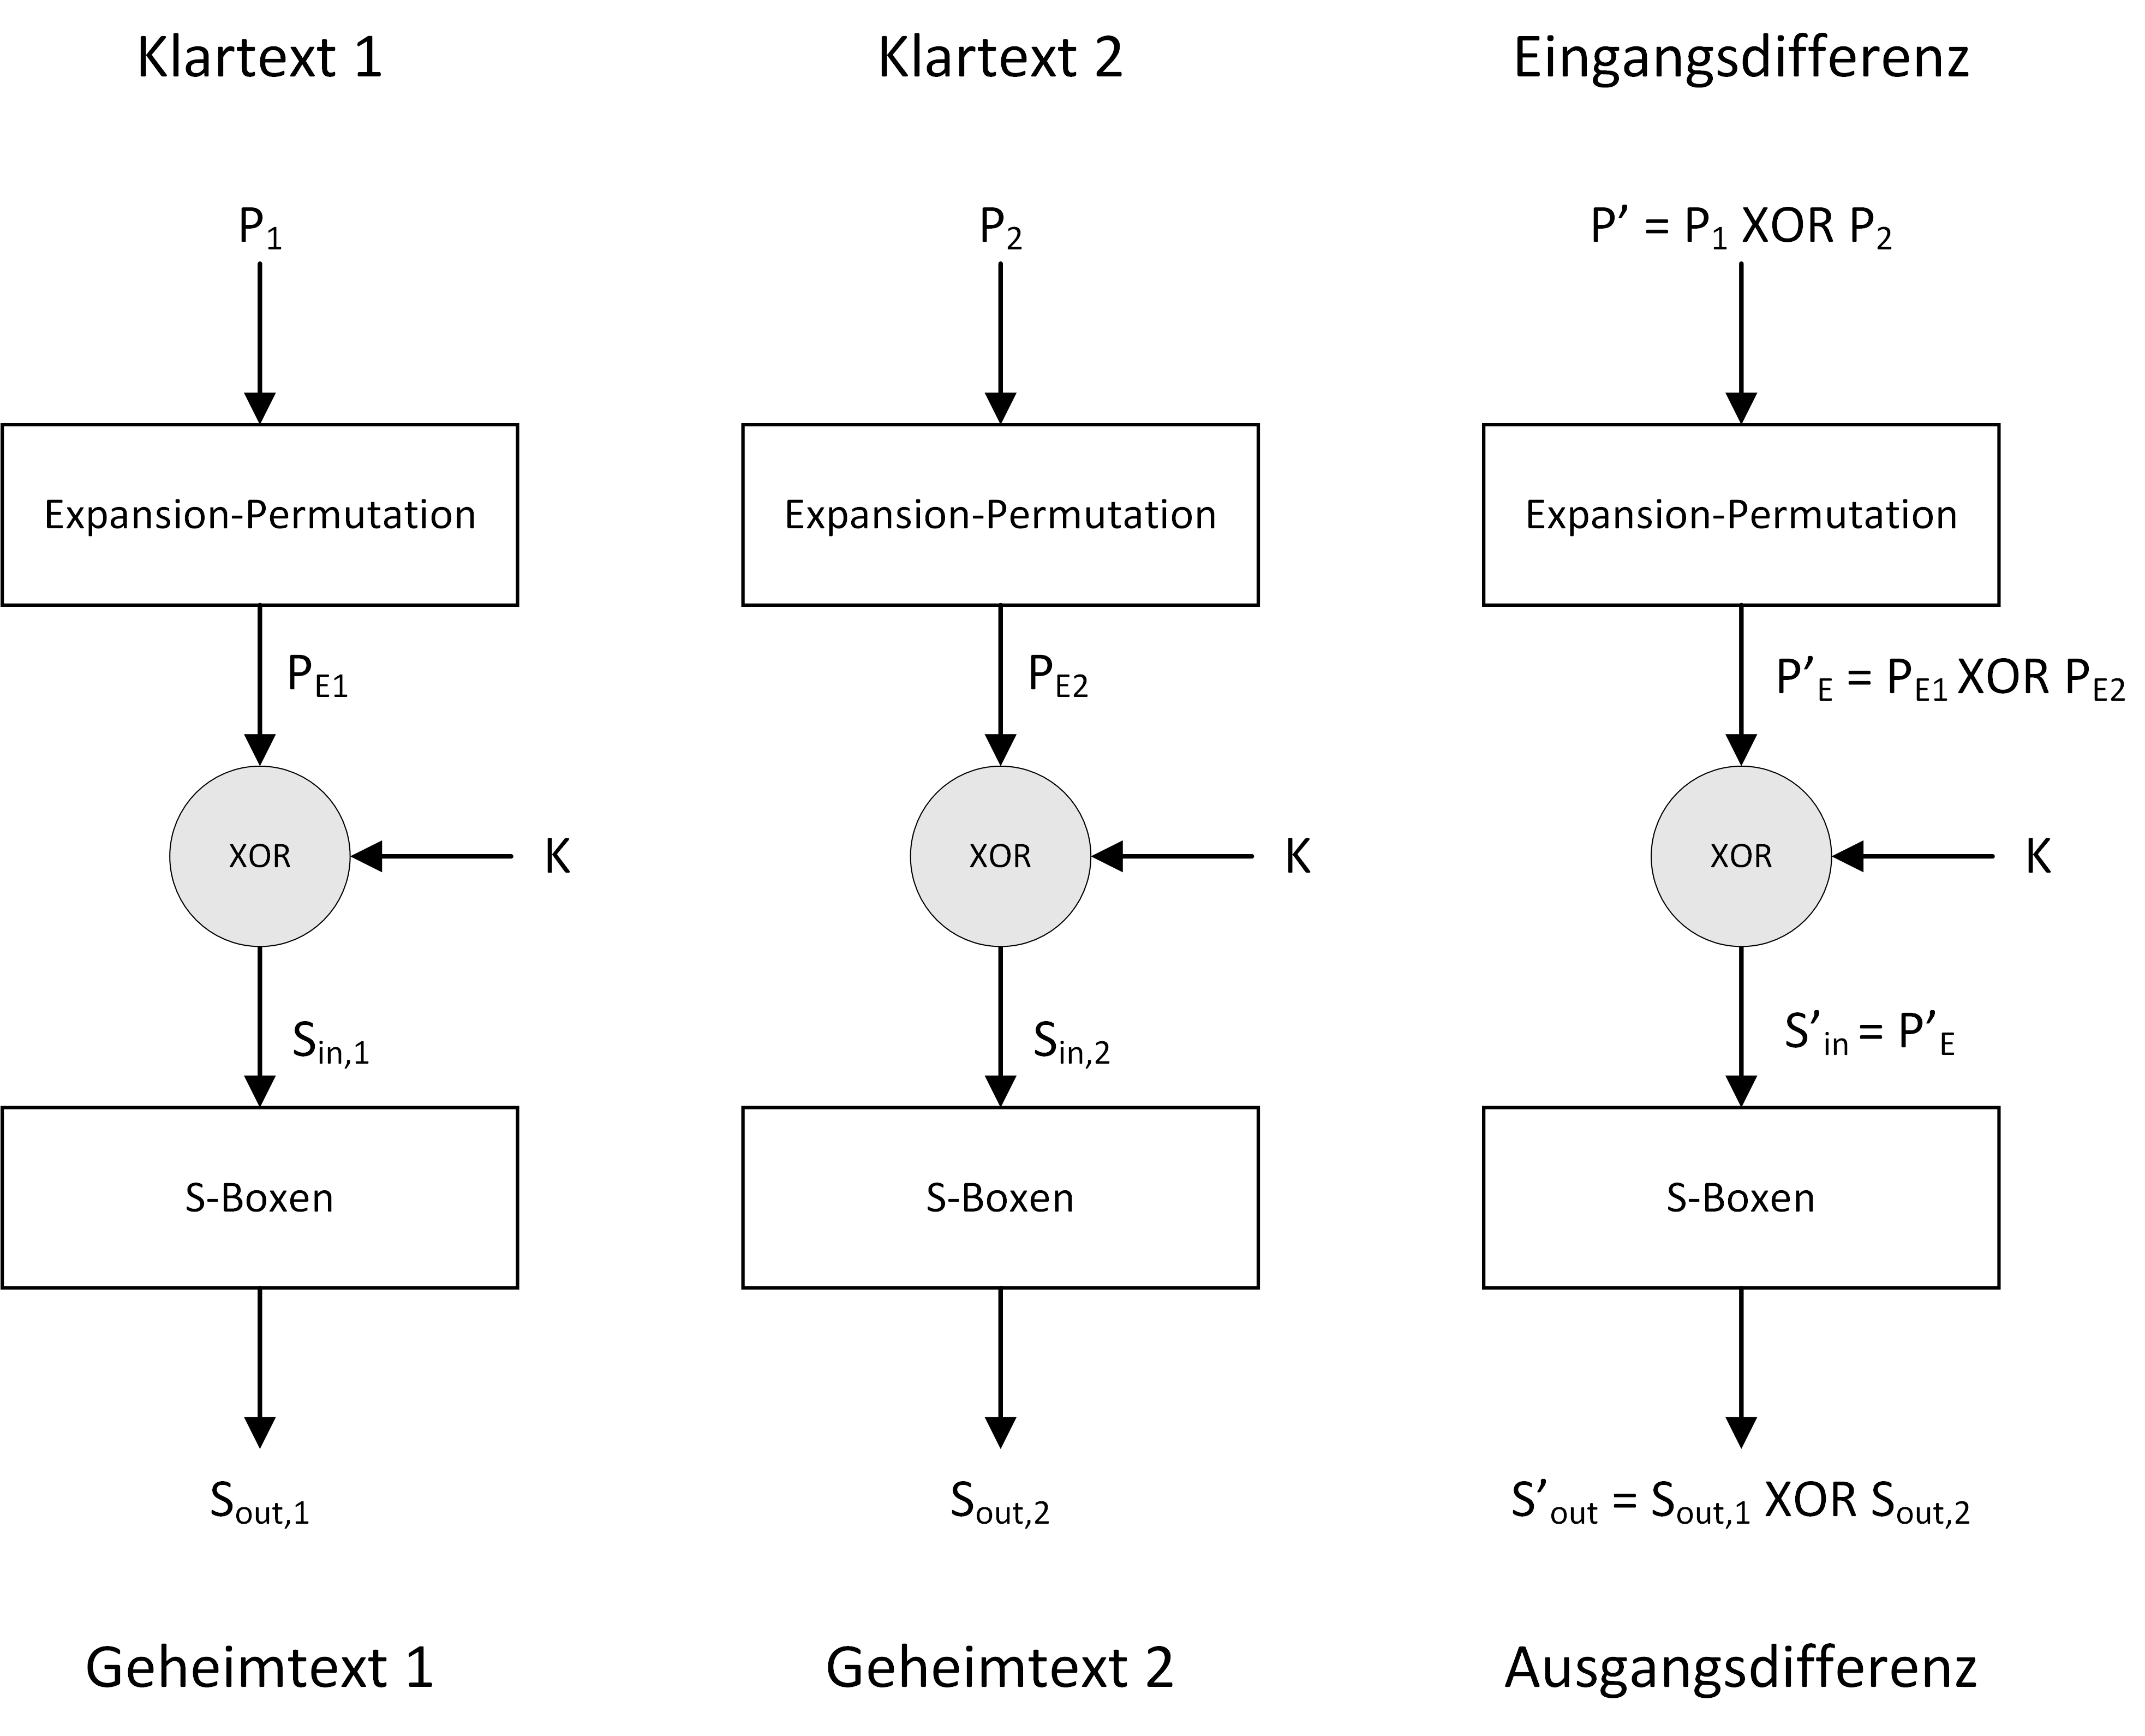
\includegraphics[width=1.0\linewidth]{graphics/DES_Differenz.jpg}
	\caption{Verhalten von Klartext 1, 2 und der Differenz davon durch die Feistelstruktur einer Runde von DES \cite{the_morpheus_tutoials_kryptographie_2016}}
	\label{fig:DES_Differenz}
\end{figure}

Die Eingangswerte $S_{in,1}$ und $S_{in,2}$ der S-Boxen sind ohne Schlüssel nicht bekannt. Bei der Spalte \glqq Differenz\grqq{} ist dieser Eingang $S'_{in}$ aber bekannt. Eine doppelte XOR-Verknüpfung mit dem Schlüssel hebt sich auf. Mit anderen Worten ist: 

\begin{equation}\label{equ:Schluessel_Differenz}
S'_{in} = S_{in,1} \oplus S_{in,2} = (P_{E,1} \oplus K) \oplus (P_{E,2} \oplus K) = P_{E,1} \oplus P_{E,2} = P'_{E} 
\end{equation}


Mit dieser Eigenschaft können die S-Boxen genauer analysiert werden. 
Wie bereits in der Einleitung erwähnt, sind die acht S-Boxen nicht-lineraren Funktion. Um diese zu umgehen kann mit Wahrscheinlichkeiten gearbeitet werden.
Anhand der öffentlich zugänglichen S-Boxen kann eine Differenzenverteilungstabelle aufgestellt werden. In dieser wird für jede Eingangsdifferenz die Zahl Wertepaar gegeben welche eine bestimmte Ausgangsdifferenz erzeugen. 
Es gibt bei DES $2^{6} = 64$ verschieden mögliche Eingangsdifferenzen pro S-Box. Jede Eingangsdifferenz kann mit 64 verschiedenen Wertepaare erzeugt werden. Als Beispiel: für eine Eingangsdifferenz von $34_{h}$ (Hexadezimalzahl) gibt es laut Differenzenverteilungstabelle nur zwei von den 64 Wertepaar die, beim Durchqueren der S-Boxen 1, eine Ausgangsdifferenz von $04_{h}$ erzeugen \cite{noauthor_differenzielle_2019}\cite{biham_differential_1990}. 

Da bei einer chosen plaintext attack die Ausgangsdifferenz bekannt ist, können die möglichen Eingangswertepaare $(S_{in,1}, S_{in,2})$ in einer weiteren Tabelle abgelesen werden. Entsprechend der Differenzenverteilungstabelle gibt es mehr oder weniger solche möglichen Eingangspaar.
Für das Beispiel mit der Eingangsdifferenz $34_{h}$ und der Ausgangsdifferenz $04_{h}$ gibt es die 2 Wertepaare $(S_{in,1}, S_{in,2}) = (13_{h}, 27_{h})$ oder $(S_{in,1},S_{in,2}) = (27_{h}, 13_{h})$. Wäre die Ausgangsdifferenz $02_{h}$ bei einer Eingangsdifferenz von $34_{h}$ würde es 16 mögliche Wertepaare geben. 

Da nun die Eingangswerte bekannt sind, kann der Schlüssel wie folgt berechnet werden:
\begin{equation}\label{equ:Schluessel_Loesung}
K = P_{E,1} \oplus S_{in,1} = P_{E,2} \oplus S_{in,2}
\end{equation}

Weil nicht mit Sicherheit gesagt werden kann welches Wertepaar $(S_{in,1}, S_{in,2})$ das richtige ist, gibt es bei diesem Beispiel zwei mögliche Schlüssel. Es müssten die anderen S-Boxen betrachtet oder mehrere Durchgänge durchgeführt werden, um den falschen Schlüssel auszuschliessen. 

\subsection{Mehrere Runden von DES}\label{subsec:Mehrere_Runden}
Bis jetzt wurde lediglich eine Runde von DES betrachtet. Es braucht nur wenige Klartext-Geheimtext-Paare damit der Schlüssel für eine Runde ermittelt werden kann. Bei mehr als 2 Runden von DES können nicht mehr alle wichtigen Differenzen in der Feistelstruktur ermittelt werden. 
An dieser Stelle kommen die Runden-Charakteristik ins Spiel. Da die Zwischenresultate nicht zur Verfügung stehen, werden sich wiederholende Strukturen gesucht, sogenannte iterative Charakteristiken. Diese können sich nach eine oder mehrere Runden wiederholen. Die Abbildung \ref{fig:Charakteristik} zeigt eine Zweirunden-Charakteristik. 

\begin{figure}[h]
	\centering
	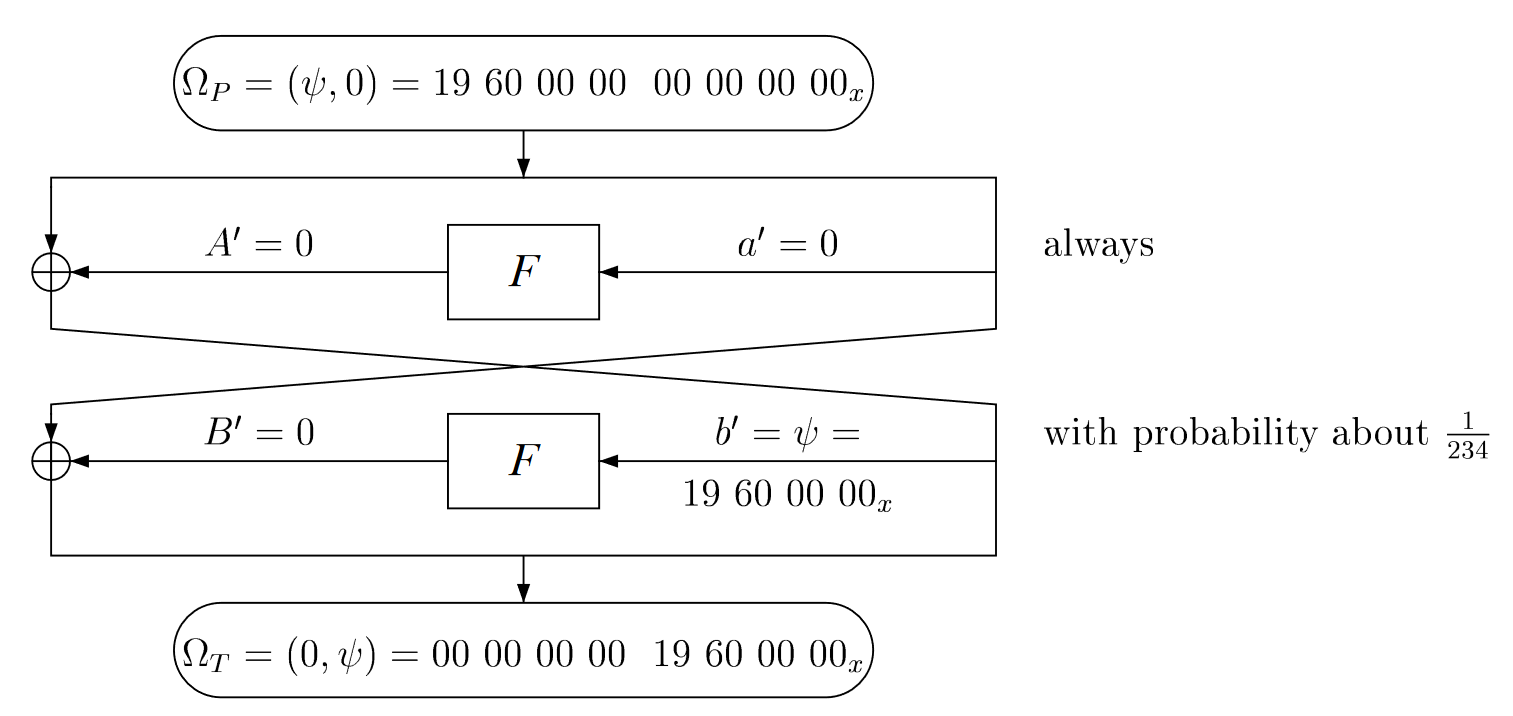
\includegraphics[width=1.0\linewidth]{graphics/Charakteristik.png}
	\caption{Dies ist eine Zweirunden-Charakteristik für die differenzielle Kryptoanalyse bei mehr als zwei Runden von DES. Die Eingangsdifferenz wiederholt sich nach zwei Runden in der Feistelstruktur \cite{biham_differential_1990}.}
	\label{fig:Charakteristik}
\end{figure}

Die Wahrscheinlichkeiten (im Bild \ref{fig:Charakteristik} auf der rechten Seite: $p_{1} = 1$ = always und $P_{2} = 1/234$) stammen aus den Differenztabellen für alle 8 S-Boxen. Anders gesagt, gibt es eine Eingangsdifferenz von 234 welche am Ausgang die selbe Differenz hat. Falls diese gefunden wird, kann in der Feistelstruktur zurück gerechnet werden und die Rundenschlüssel somit ermittelt werden. 
Es gibt andere Eingangsdifferenzen welche sich nach zwei Runden wiederholen, entsprechend nicht nur $\Omega_{P} = 19600000\ 00000000$,  jedoch sind diese eher selten. Die meisten davon sind gut bei wenig Runden von DES (bis 9 Runden).
Das Beipiel in Abbildung \ref{fig:Charakteristik} kann aber bis 15 Runden von DES gebraucht werden. 
Umso mehr Runden der Verschlüsselungsalgorithmus hat, desto unwahrscheinlicher ist es ein richtiges Paar zu finden. Die Wahrscheinlichkeiten der Charakteristiken werden miteinander Multipliziert.
Bei 16 Runden wird die Wahrscheinlichkeit das richtige Paar zu finden so klein, dass ein Brut-force Attacke genau so schneller wäre.
Die differenzielle Kryptoanalyse ist hingegen effizient bei anderen DES-ähnliche Kryptosysteme. Verschlüsselungsverfahren wie die Achtrunden-Variante von Lucifer (Verschlüsselungsverfahren entworfen durch IBM vor DES) oder FEAL-4 / FEAL-8 können zum Beispiel mit der vorgestellten Methode gebrochen werden. FEAL mit weniger als 32 Runden können teilweise gebrochen werden \cite{biham_differential_1990}.














%\clearpage
\section{Anwendung}\label{sec:Anwendung}
In der Funktionsweise wurde bis jetzt lediglich eine Runde von DES durchgelaufen. Es braucht nur wenige Klartext-Geheimtext Paare damit der Schlüssel für eine Runde ermittelt werden kann. 
Biham und Shamir haben weiter gezeigt, dass die Differenzielle Kryptoanalyse auf 2 Runden und mehr erweitert werden kann, doch umso höher die Anzahl Runden desto schwieriger die Entschlüsselung. Es muss mit den Wahrscheinlichkeiten aus der Differenzenverteilungstabelle weiter gerechnet werden. 
Bei 16 Runden wird die Wahrscheinlichkeit den richtigen Schlüssel zu finden so klein, dass ein Brut-force Attacke genau so schneller wäre.
Die differenzielle Kryptoanalyse ist hingegen effizient bei anderen DES-ähnliche Kryptosysteme. Verschlüsselungsverfahren wie die achtrunden Variante von Lucifer (Verschlüsselungsverfahren entworfen durch IBM vor DES) oder FEAL-4 / FEAL-8 können zum Beispiel mit der vorgestellten Methode gebrochen werden. FEAL mit weniger als 32 Runden können teilweise gebrochen werden \cite{biham_differential_1990}.
















%\clearpage
\section{Schluss}\label{sec:Schluss}











\pagebreak


%\clearpage
%%---BIBLIOGRAPHY------------------------------------------------------------------------


{\sloppypar
%\printbibliography[heading=bibnumbered ]
\label{sec:lit}
\selectlanguage{ngerman}				%ngerman or english
\printbibliography
}

%\pagebreak

%\input{sections/8_0_Ehrlichkeitserklaerung}
%\pagebreak
%%---APPENDIX----------------------------------------------------------------------------
%\appendix
%%\begin{appendix} %Anhang


%Anhang A
%\includepdf[pages={1},nup=1x1,landscape=false,scale=0.90, pagecommand = \section*{\LARGE{Anhang:}}
%\addcontentsline{toc}{section}{Anhang}
%\section{Auftrag des Arbeitgebers}
%\label{app:Lastenheft}, offset =0mm -22mm ]{appendix/Lastenheft.pdf}\newpage
%Bei mehrseitigen Dokumenten die folgenden Seiten ohne Überschrift:
%\includepdf[pages={2},nup=1x1,landscape=false,scale=0.90,offset=6 -30,pagecommand={\thispagestyle{myheadings}}]{appendix/Lastenheft.pdf} 
%\newpage


%Anhang B: Bestimmung der Ersatzelemente der ASM
%\input{sections/ASM_Laborjournal}


%Anhang C: Messungen für ADC-Verifikation
\clearpage
\section{Messungen Zeitverzögerung Modulator}\label{app:Messungen_Delay Modulator}



\begin{figure}[H]
	\centering
	\includegraphics[width=0.85\linewidth]{appendix/Delay_modulator.png}
	\caption{Messung der Zeitverzögerung zwischen Modulatoreingang und modulierter Spannung an der ASM}
	\label{fig:app_delay}
\end{figure}


%Beispiel für A3 Seite einfügen:

%Anhang B
%A3
%\eject\pdfpagewidth=420mm \pdfpageheight=297mm
%A3


%Anhang B: Schema Layout
%\includepdf[pages={1},nup=1x1,landscape=false,scale=1.7,offset=300 -50,pagecommand={\section{Schema BMS-Slave}\label{app: Schema_Layout}\thispagestyle{myheadings}}]{appendix/Schema_Layout_.pdf} \newpage

%A4
%\eject\pdfpagewidth=210mm \pdfpageheight=297mm
%A4


%Beispiel Anhang C: (PDF)



%Anhang C: Dimensionierung passives Balancing
%\includepdf[pages={1},nup=1x1,landscape=false,scale=0.90,offset=10 -40,pagecommand={\section{Dimensionierung passives Balancing}\label{app: Dimensionierung_Balancing}\thispagestyle{myheadings}}]{appendix/Dimensionierung_Balancing.pdf} 
%\newpage


%\end{appendix}


%%---NOTES for DEBUG---------------------------------------------------------------------
%\ifdraft{%Do this only if mode=draft
%\usepackage{todonotes})
%\newpage
%\listoftodos[\section{Todo-Notes}]
%\clearpage
%}
%

\end{document}
